% Introdução

\documentclass[_ArquivoPrincipal.tex]{subfiles}

\begin{document}

%==================================================================================================
\chapter{Introdução}
%==================================================================================================

Visto o constante avanço da engenharia em poder se dimensionar estruturas cada vez mais leves e esbeltas, observa-se a necessidade de uma determinação cada vez mais precisa de todos os parâmetros que podem influenciar na resistência e estabilidade da estrutura. Nesse contexto torna-se de grande importância a verificação dos efeitos da interação entre os fluidos e a estrutura, uma vez que esses fenômenos podem comprometer a segurança estrutural. Exemplos de problemas envolvendo Interação Fluido-Estrutura (IFE) podem ser notados em ações do vento sobre estruturas de grandes altitudes, ação de marés sobre estruturas de barragens e estruturas \textit{offshore}, dentre outros. Além disso, também percebe-se a aplicação desse tipo de análise em demais áreas, como, por exemplo, no estudo de escoamento do sangue em vasos sanguíneos, ou em problemas envolvendo aerodinâmica \cite{sanches2014fluid, fernandes2020tecnica}.

Desse modo, é possível realizar a análise de IFE de duas formas principais: a construção de amostras em escala; ou a modelagem matemática do problema em questão. No primeiro caso há a verificação real do comportamento da estrutura e do fluido à um determinado problema. No entanto, dependendo da natureza do problema, esse comportamento pode variar de acordo com a escala, o que pode não apresentar resultados representativos. Também ressalta-se o fato de a contrução das amostras demandar uma infraestrutura robusta para se analisar apenas alguns problemas específicos \cite{fernandes2020tecnica}.

Já a modelagem matemática de problemas se mostra como uma opção mais viável para análise de problemas de IFE, uma vez que dispensa grandes investimentos e possui grande flexibilidade de aplicações, podendo ser utilizado em diversos tipos de análises. Porém, em muitos casos, o estudo matemático de IFE leva a modelagem de problemas muito complexos, com alto custo computacional, exigindo, assim, formulações mais robustas para sua aplicação.

\textcolor{red}{COMENTAR SOBRE TURBULÊNCIA}

Para se realizar o estudo, tanto da mecânica dos elementos sólidos, quanto para a meĉanica dos fluidos, é necessário o estabelecimento de algumas simplificações. Uma das principais simplificações utilizada para esses problemas é a que considera os objetos de análise como meios contínuos, desprezando-se, dessa forma, os efeitos advindos da microestrutura da matéria \cite{lai2009introduction, mase2009continuum}.

Sabe-se que toda a matéria é composta por átomos e partículas subatômicas, no entanto a mecânica do contínuo desconsidera os efeitos dessas partículas e aponta que todo material pode ser subdividido em elementos cada vez menores sem que haja mudanças em suas propriedades físicas, independentemente do quão pequena seja essa divisão. Assim, faz-se possível a modelagem de elementos com volume infinitesimal, permitindo a utilização de artifícios matemáticos, como o cálculo diferencial e integral. Dessa forma, teorias baseadas na elasticidade e plasticidade podem ser empregadas utilizando funções contínuas, facilitando a determinação de parâmetros de interesse da análise \cite{irgens2008continuum, lai2009introduction, malvern1969introduction}.

Vale ressaltar que a consideração dos meios contínuos apresenta resultados muito satisfatórios nos estudos de engenharia, uma vez que os objetos de estudo possuem dimensões muito maiores que as distâncias moleculares do mesmo \cite{malvern1969introduction, mase2009continuum}.

Ainda existem diferentes formas de descrever matematicamente um problema mecânico, em termos da referência adotada para os cálculos. São estas: a descrição Lagrangiana (ou material) e a descrição Euleriana (ou espacial).

Na descrição Lagrangiana a referência adotada é a configuração inicial do contínuo (denotada por $\mathbf{x}$). Essa descrição apresenta boa representatividade quando aplicada em modelos sólidos, uma vez que a configuração inicial dos elementos é bem definida, tendo como variáveis principais os deslocamentos do elemento \cite{sanches2014fluid, fernandes2019ale}.

Já a descrição Euleriana toma como referência a configuração atual do contínuo (denotada por $\mathbf{y}$), sendo bem utilizada para a descrição de fluidos newtonianos, pois estes não apresentam resistência à esforços de cisalhamento, distorcendo-se indefinidamente quando submetidos à tais esforços. Nesse tipo de descrição é comum a utilização para determinação de velocidades, diferentemente dos deslocamentos \cite{sanches2014fluid, fernandes2019ale}.

%==================================================================================================
\section{Acomplamento ALE} \label{ALE}
%==================================================================================================

A descrição Lagrangiana-Euleriana Arbitrária (\textit{Arbitrary Lagrangian-Eulerian} - ALE), é uma forma de analisar os pontos de um contínuo em termos de uma região arbitrária do espaço. Esse estudo foi introduzido inicialmente por \citeonline{donea1982arbitrary} e busca descrever a movimentação do contínuo a partir de uma generalização das descrições Lagrangiana e Euleriana. Na descrição Lagrangiana, a análise é realizada tomando-se como referência a posição inicial do contínuo, podendo ser atualizada para acompanhar esse movimento, enquanto a descrição Euleriana a análise é feita tomando-se como referência a posição atual do contínuo, sendo, então, uma posição fixa no espaço. Assim, a descrição ALE, ao contrário da Lagrangiana e Euleriana, busca analisar esse movimento a partir de uma região do espaço que pode se movimentar independentemente das configurações do contínuo.

A Figura \ref{fig:ALE} apresenta um desenho esquemático das regiões ocupadas pelo contínuo na sua configuração inicial, atual e a região de referência.

\begin{figure}[h]
    \centering
    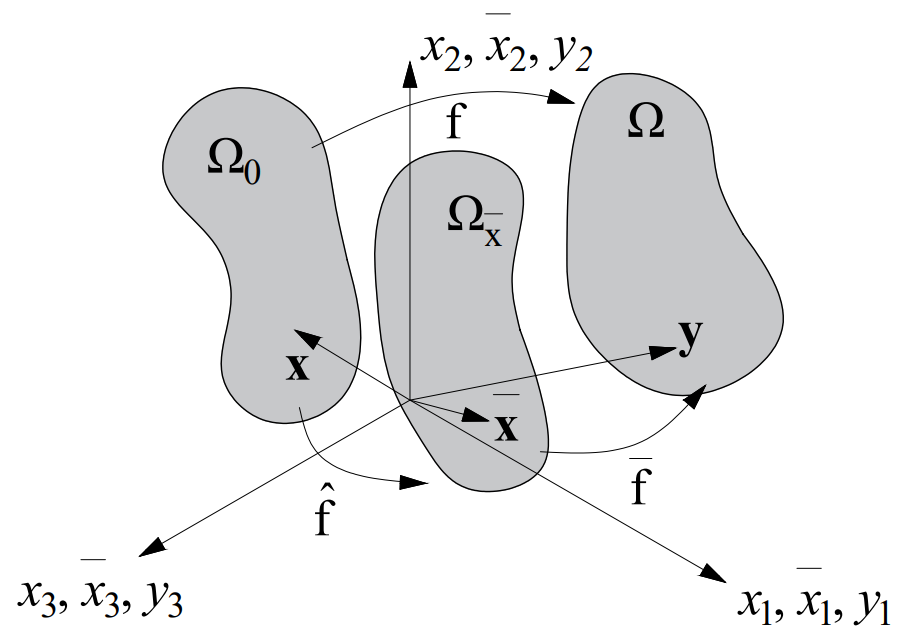
\includegraphics[width=0.5\linewidth]{Figuras/ALE1.png}
    \caption{Representação esquemática da descrição ALE.}
    \label{fig:ALE}
\end{figure}

%==================================================================================================
\section{Objetivos}
%==================================================================================================

\textcolor{red}{OBJETIVOS}

\begin{itemize}
    \item ITEM 1;

    \item ITEM 2;

    \item ITEM 3;

    \item ITEM 4.
\end{itemize}

%==================================================================================================
\section{Justificativa}
%==================================================================================================

\textcolor{red}{JUSTIFICATIVA}

\end{document}